\documentclass[11pt,a4paper]{article}

\usepackage[utf8]{inputenc}
\usepackage[T1]{fontenc}
\usepackage[english]{babel}
\usepackage[margin=25mm]{geometry}
\usepackage{amsmath,amssymb}
\usepackage{siunitx}
\usepackage{booktabs}
\usepackage{listings}
\usepackage{xcolor}
\usepackage{tikz}
\usetikzlibrary{positioning,arrows.meta,fit,backgrounds,calc,shapes.geometric}
\usepackage{hyperref}

\sisetup{detect-all, per-mode=symbol}

\lstset{
  basicstyle=\ttfamily\small,
  frame=single,
  breaklines=true,
  columns=fullflexible,
  keepspaces=true
}

\title{Aging Estimation of an IGBT-Based Drive\\
\large Arrhenius model with joint current and coolant temperature thresholds}
\author{}
\date{\today}

\begin{document}
\maketitle

\section{Scope and assumptions}

This document defines an empirical model for the cumulative aging estimation of
a liquid-cooled drive, based on quantities available online:

\begin{itemize}
  \item delivered current $I$ (phase RMS value);
  \item heatsink inlet water temperature $T_w$;
  \item IGBT junction temperature $T_j$ (measured or estimated);
  \item number of maintenance or repair interventions $N$ performed on the
        drive;
  \item IGBT module type, $\tau \in \{1,2\}$.
\end{itemize}

The approach follows the physics-of-failure framework commonly used for
reliability assessment of power converters~\cite{wang2013,ma2016,lutz2018}.

Base assumptions:

\begin{enumerate}
  \item the dominant degradation mechanism is thermally activated, hence
        describable by an Arrhenius law on junction temperature;
  \item current acts as a multiplicative stress factor (losses, current density
        in the bond wires, thermal cycle amplitude);
  \item an \emph{out-of-design} operating condition exists when the coolant
        temperature exceeds a threshold \emph{simultaneously} with the current
        exceeding a threshold; in that condition the aging rate is further
        accelerated;
  \item the type~1 module has an aging coefficient twice that of the type~2
        module;
  \item each maintenance intervention leaves a residual penalty (reassembly,
        thermomechanical stress on the power stack, degradation of the thermal
        interface).
\end{enumerate}

\section{Notation}

\begin{table}[h]
\centering
\begin{tabular}{llc}
\toprule
Symbol & Meaning & Unit \\
\midrule
$I$            & delivered current (RMS)                             & \si{\ampere} \\
$I_N$          & rated drive current                                 & \si{\ampere} \\
$I_{th}$       & current threshold for the accelerated regime        & \si{\ampere} \\
$T_w$          & inlet water temperature                             & \si{\degreeCelsius} \\
$T_{w,th}$     & water temperature threshold                         & \si{\degreeCelsius} \\
$T_j$          & IGBT junction temperature                           & \si{\kelvin} \\
$T_{ref}$      & model reference temperature                         & \si{\kelvin} \\
$E_a$          & activation energy                                   & \si{\electronvolt} \\
$k_B$          & Boltzmann constant, \num{8.617e-5}                  & \si{\electronvolt\per\kelvin} \\
$m$            & current stress exponent                             & -- \\
$\beta$        & acceleration gain in the threshold regime           & -- \\
$\gamma$       & penalty per maintenance intervention                & -- \\
$k_\tau$       & aging coefficient of the module type                & -- \\
$L_0$          & expected life at reference conditions               & \si{\hour} \\
$A$            & cumulative aging index, $A\in[0,1]$                 & -- \\
\bottomrule
\end{tabular}
\caption{Symbols used in the document.}
\end{table}

\section{Model overview}
\label{sec:schema}

Figure~\ref{fig:schema} summarises the model structure: measured quantities on
the left, acceleration factors in the centre, damage accumulator and diagnostic
outputs on the right.

\begin{figure}[htbp]
\centering
\resizebox{\textwidth}{!}{%
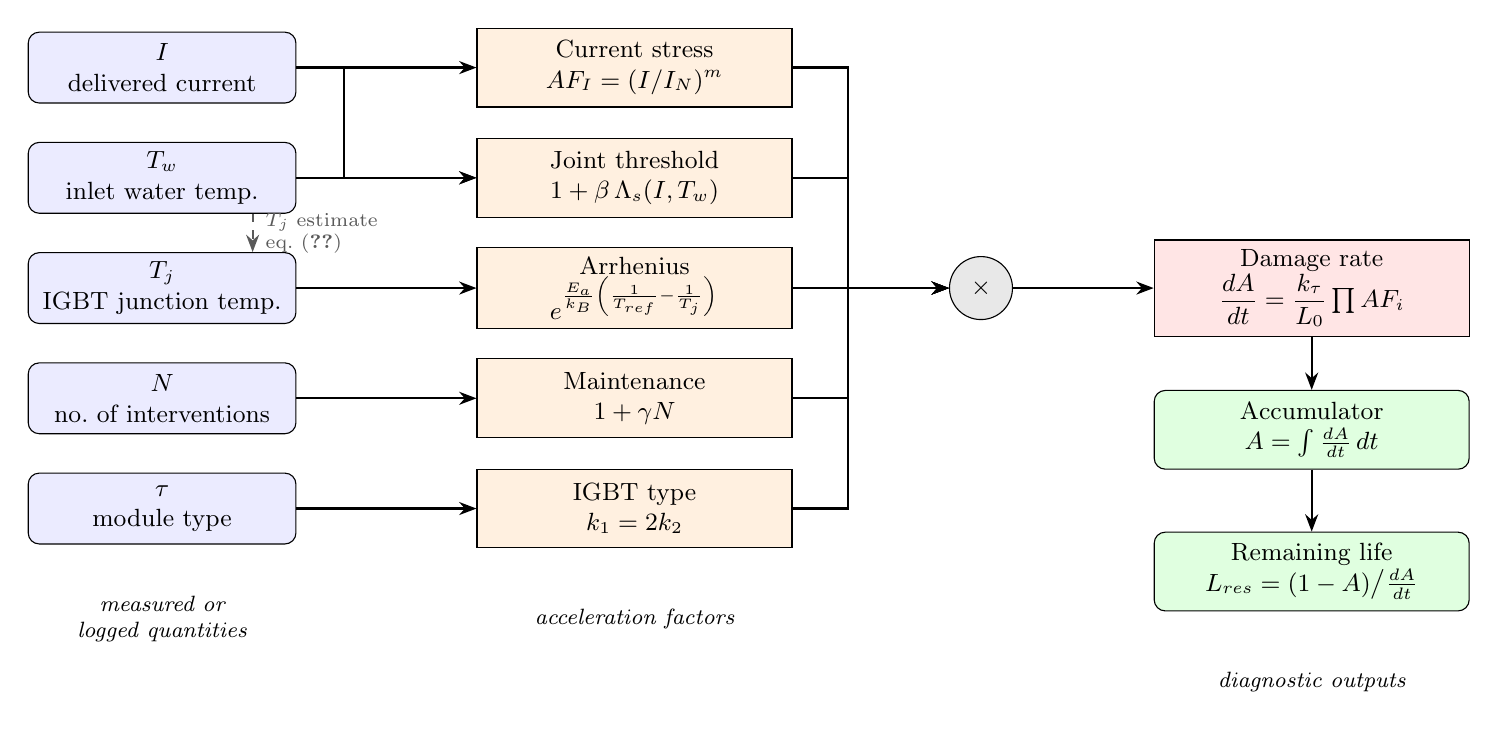
\begin{tikzpicture}[
  font=\small,
  inp/.style={draw, rounded corners, fill=blue!8, minimum width=34mm,
              minimum height=9mm, align=center},
  blk/.style={draw, fill=orange!12, minimum width=40mm,
              minimum height=10mm, align=center},
  outb/.style={draw, rounded corners, fill=green!12, minimum width=40mm,
              minimum height=10mm, align=center},
  op/.style={draw, circle, fill=gray!18, inner sep=0.5pt, minimum size=8mm},
  ar/.style={-{Stealth[length=2.2mm]}, thick},
  dar/.style={-{Stealth[length=2.2mm]}, thick, dashed, gray!70!black}
]

%% ---- inputs ----
\node[inp] (I)   at (0, 4.6) {$I$\\delivered current};
\node[inp] (Tw)  at (0, 3.2) {$T_w$\\inlet water temp.};
\node[inp] (Tj)  at (0, 1.8) {$T_j$\\IGBT junction temp.};
\node[inp] (N)   at (0, 0.4) {$N$\\no.\ of interventions};
\node[inp] (TY)  at (0,-1.0) {$\tau$\\module type};

%% ---- acceleration factors ----
\node[blk] (AFI)  at (6.0, 4.6) {Current stress\\$AF_I=(I/I_N)^m$};
\node[blk] (LAM)  at (6.0, 3.2) {Joint threshold\\$1+\beta\,\Lambda_s(I,T_w)$};
\node[blk] (ARR)  at (6.0, 1.8) {Arrhenius\\$e^{\frac{E_a}{k_B}\left(\frac{1}{T_{ref}}-\frac{1}{T_j}\right)}$};
\node[blk] (AFN)  at (6.0, 0.4) {Maintenance\\$1+\gamma N$};
\node[blk] (KT)   at (6.0,-1.0) {IGBT type\\$k_1=2k_2$};

%% ---- product and outputs ----
\node[op]  (MUL)  at (10.4, 1.8) {$\times$};
\node[blk, fill=red!10] (RATE) at (14.6, 1.8)
     {Damage rate\\$\dfrac{dA}{dt}=\dfrac{k_\tau}{L_0}\prod AF_i$};
\node[outb] (INT)  at (14.6, 0.0) {Accumulator\\$A=\int \frac{dA}{dt}\,dt$};
\node[outb] (RES)  at (14.6,-1.8) {Remaining life\\$L_{res}=(1-A)\big/\frac{dA}{dt}$};

%% ---- connections ----
\draw[ar] (I)  -- (AFI);
\draw[ar] (Tw) -- (LAM);
\draw[ar] (Tj) -- (ARR);
\draw[ar] (N)  -- (AFN);
\draw[ar] (TY) -- (KT);
\draw[ar] (I.east) -- ++(0.6,0) |- (LAM.west);
\draw[dar] ($(Tw.south)+(1.15,0)$) -- ($(Tj.north)+(1.15,0)$)
      node[midway, right=1pt, font=\scriptsize, align=left]
      {$T_j$ estimate\\eq.~\eqref{eq:termico}};

\foreach \n in {AFI,LAM,ARR,AFN,KT}{
  \draw[ar] (\n.east) -- ++(0.7,0) |- (MUL);
}
\draw[ar] (MUL) -- (RATE);
\draw[ar] (RATE) -- (INT);
\draw[ar] (INT) -- (RES);

%% ---- captions inside the figure ----
\node[align=center, font=\footnotesize\itshape] at (0,-2.4) {measured or\\logged quantities};
\node[align=center, font=\footnotesize\itshape] at (6.0,-2.4) {acceleration factors};
\node[align=center, font=\footnotesize\itshape] at (14.6,-3.2) {diagnostic outputs};

\end{tikzpicture}}
\caption{Structure of the aging estimation model: measured inputs generate
multiplicative acceleration factors which, combined with the module type
coefficient $k_\tau$, define the life consumption rate; time integration yields
the cumulative index and the remaining life.}
\label{fig:schema}
\end{figure}

Figure~\ref{fig:soglie} shows the operating plane $(I,T_w)$ with the critical
quadrant where the additional acceleration factor is activated: activation
requires the two thresholds to be exceeded \emph{simultaneously}.

\begin{figure}[htbp]
\centering
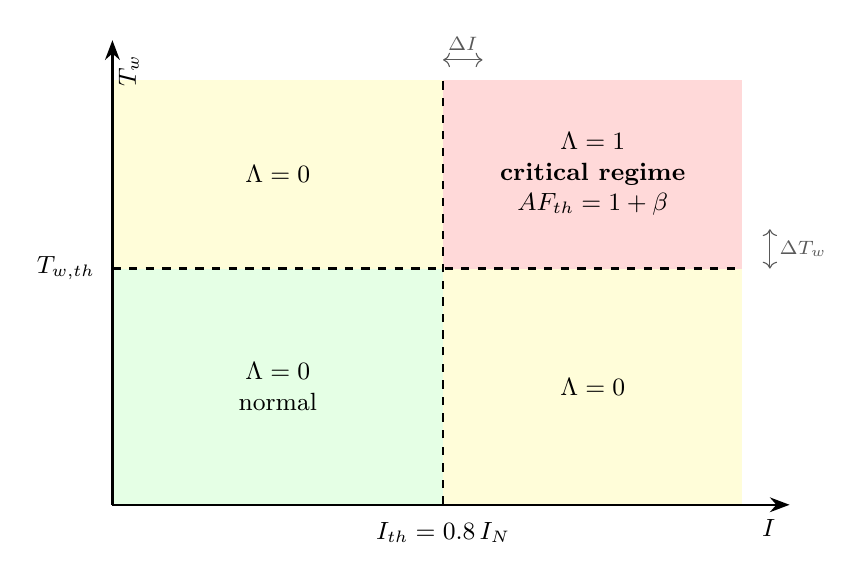
\begin{tikzpicture}[font=\small, scale=1.0]

% critical area
\fill[red!15] (4.2,3.0) rectangle (8.0,5.4);
% non-critical areas
\fill[green!10] (0,0) rectangle (4.2,3.0);
\fill[yellow!15] (4.2,0) rectangle (8.0,3.0);
\fill[yellow!15] (0,3.0) rectangle (4.2,5.4);

% threshold lines
\draw[dashed, thick] (4.2,0) -- (4.2,5.4);
\draw[dashed, thick] (0,3.0) -- (8.0,3.0);

% axes
\draw[-{Stealth[length=2.5mm]}, thick] (0,0) -- (8.6,0) node[below left=2pt] {$I$};
\draw[-{Stealth[length=2.5mm]}, thick] (0,0) -- (0,5.9) node[below left=2pt, rotate=90] {$T_w$};

\node[below] at (4.2,-0.1) {$I_{th}=0.8\,I_N$};
\node[left]  at (-0.1,3.0) {$T_{w,th}$};

\node[align=center, font=\small] at (2.1,1.5) {$\Lambda=0$\\normal};
\node[align=center, font=\small] at (6.1,1.5) {$\Lambda=0$};
\node[align=center, font=\small] at (2.1,4.2) {$\Lambda=0$};
\node[align=center, font=\small\bfseries] at (6.1,4.2)
     {$\Lambda=1$\\critical regime\\$AF_{th}=1+\beta$};

% regularised transition widths
\draw[<->, gray!70!black] (4.2,5.65) -- (4.7,5.65)
      node[midway, above, font=\scriptsize] {$\Delta I$};
\draw[<->, gray!70!black] (8.35,3.0) -- (8.35,3.5)
      node[midway, right, font=\scriptsize] {$\Delta T_w$};

\end{tikzpicture}
\caption{Current versus water temperature operating plane. The additional
acceleration factor is activated only in the upper-right quadrant; $\Delta I$
and $\Delta T_w$ are the transition widths of the regularised
formulation~\eqref{eq:lambda_soft}.}
\label{fig:soglie}
\end{figure}

\section{Simplified thermal model}

If $T_j$ is not available from direct measurement (module NTC, $V_{ce,on}$ used
as a thermo-sensitive electrical parameter~\cite{avenas2012}), it can be
estimated in quasi-steady-state conditions from $T_w$ and the losses:

\begin{equation}
  T_j = T_w + R_{th,jw}\,P_{loss}(I),
  \qquad
  P_{loss}(I) \simeq a_1 I + a_2 I^2 ,
  \label{eq:termico}
\end{equation}

where the linear term represents the switching losses (approximated as
proportional to the switched current) and the quadratic term the conduction
losses across the differential resistance. $R_{th,jw}$ includes
junction-to-case, thermal interface and case-to-water contributions, and is a
function of the coolant flow rate.

\section{Arrhenius acceleration factor}

The acceleration factor with respect to the reference temperature is

\begin{equation}
  AF_{Arr}(T_j) = \exp\!\left[\frac{E_a}{k_B}
  \left(\frac{1}{T_{ref}} - \frac{1}{T_j}\right)\right].
  \label{eq:arrhenius}
\end{equation}

For $T_j > T_{ref}$ we get $AF_{Arr} > 1$ (accelerated aging), for
$T_j < T_{ref}$ we get $AF_{Arr} < 1$. Temperatures must be expressed in
kelvin. Typical $E_a$ values for power modules range between
\SI{0.4}{\electronvolt} and \SI{0.8}{\electronvolt} depending on the dominant
mechanism (metallisation degradation, electromigration, gel
degradation)~\cite{ciappa2002,jep122}.

\section{Current stress factor}

\begin{equation}
  AF_I(I) = \left(\frac{I}{I_N}\right)^{m},
  \qquad m \in [1.5,\,4].
  \label{eq:corrente}
\end{equation}

The exponent $m$ captures, in compact form, the dependence of damage on thermal
cycle amplitude (Coffin--Manson type, $N_f \propto \Delta T_j^{-n}$, with
$\Delta T_j$ increasing with $I$). Reference power cycling lifetime models for
IGBT modules are LESIT~\cite{held1997}, CIPS08~\cite{bayerer2008} and
Scheuermann~\cite{scheuermann2013}.

\section{Joint threshold condition}

The accelerated aging regime is activated when \emph{both} conditions hold:

\begin{equation}
  \Lambda(I,T_w) =
  \mathbb{1}\!\left[T_w > T_{w,th}\right]\cdot
  \mathbb{1}\!\left[I > I_{th}\right] \in \{0,1\}.
  \label{eq:lambda_hard}
\end{equation}

The step formulation \eqref{eq:lambda_hard} is discontinuous and, in the
presence of measurement noise, causes repeated toggling of the index. A
regularised version based on sigmoid functions is therefore preferred:

\begin{equation}
  \Lambda_s(I,T_w) =
  \sigma\!\left(\frac{T_w - T_{w,th}}{\Delta T_w}\right)\cdot
  \sigma\!\left(\frac{I - I_{th}}{\Delta I}\right),
  \qquad
  \sigma(x) = \frac{1}{1+e^{-x}} ,
  \label{eq:lambda_soft}
\end{equation}

with $\Delta T_w$ and $\Delta I$ transition widths (for example \SI{2}{\kelvin}
and $0.05\,I_N$). Alternatively, the step form can be kept by adding hysteresis
on both thresholds.

The overall acceleration factor of the out-of-design condition is

\begin{equation}
  AF_{th}(I,T_w) = 1 + \beta\,\Lambda_s(I,T_w),
\end{equation}

where $\beta = 1$ corresponds to doubling the aging rate in the critical
regime.

\section{IGBT type}

\begin{equation}
  k_\tau =
  \begin{cases}
    2\,k_0 & \tau = 1 \quad \text{(type 1 module)}\\[2pt]
    k_0    & \tau = 2 \quad \text{(type 2 module)}
  \end{cases}
  \qquad k_0 = 1 .
  \label{eq:tipo}
\end{equation}

For the same mission profile, the type~1 module consumes life at twice the rate
of the type~2 module.

\section{Maintenance interventions}

Each intervention on the drive introduces a permanent penalty, modelled as a
linear multiplicative factor:

\begin{equation}
  AF_N(N) = 1 + \gamma N ,
  \qquad \gamma \in [0.02,\,0.10].
  \label{eq:interventi}
\end{equation}

The counter $N$ is incremented at each logged intervention (module replacement,
opening of the cooling circuit, reassembly of the power stack). To distinguish
intervention severity, $\gamma N$ can be replaced by $\sum_{i=1}^{N}\gamma_i$,
with $\gamma_i$ weighted by intervention class.

\section{Complete formulation}

The instantaneous life consumption rate is

\begin{equation}
  \boxed{\;
  \frac{dA}{dt} =
  \frac{k_\tau}{L_0}\,
  \left(\frac{I}{I_N}\right)^{m}
  \exp\!\left[\frac{E_a}{k_B}\!\left(\frac{1}{T_{ref}}-\frac{1}{T_j}\right)\right]
  \bigl[1+\beta\,\Lambda_s(I,T_w)\bigr]\,
  \bigl(1+\gamma N\bigr)\;}
  \label{eq:master}
\end{equation}

and the cumulative aging index

\begin{equation}
  A(t) = \int_{0}^{t} \frac{dA}{d\xi}\,d\xi ,
  \qquad
  A \in [0,1],
\end{equation}

with $A = 0$ for a new drive and $A = 1$ at conventional end of life. The
remaining life estimated at constant operating conditions is

\begin{equation}
  L_{res} = \frac{1 - A(t)}{\dfrac{dA}{dt}} .
\end{equation}

\section{Discrete-time implementation}

With sampling period $T_s$ (typically \SIrange{1}{60}{\second}, since thermal
dynamics are slow compared to the control loop):

\begin{equation}
  A[k+1] = A[k] + T_s\,
  \frac{k_\tau}{L_0}\,
  \left(\frac{I[k]}{I_N}\right)^{m} AF_{Arr}\bigl(T_j[k]\bigr)
  \bigl[1+\beta\Lambda_s\bigr]\bigl(1+\gamma N[k]\bigr).
\end{equation}

\begin{lstlisting}[caption={Pseudo-code for embedded implementation.}]
/* executed every Ts seconds */
Tj_K  = Tj_C + 273.15f;
af_arr = expf( (Ea/kB) * (1.0f/Tref_K - 1.0f/Tj_K) );
af_i   = powf( I/IN, m );
lam    = sigm((Tw - Tw_th)/dTw) * sigm((I - I_th)/dI);
af_th  = 1.0f + beta*lam;
af_n   = 1.0f + gamma*(float)N;
k_tau  = (igbt_type == 1) ? 2.0f : 1.0f;

rate   = (k_tau/L0) * af_i * af_arr * af_th * af_n;   /* 1/h */
A     += rate * (Ts/3600.0f);
if (A > 1.0f) A = 1.0f;
\end{lstlisting}

The accumulator $A$ must be stored in non-volatile memory at a rate compatible
with the allowed number of write cycles.

\section{Suggested parameters}

\begin{table}[h]
\centering
\begin{tabular}{lcl}
\toprule
Parameter & Value & Notes \\
\midrule
$E_a$      & \SI{0.5}{\electronvolt} & from qualification or field data \\
$T_{ref}$  & \SI{100}{\degreeCelsius} & reference junction temperature \\
$L_0$      & \SI{1e5}{\hour}          & expected life at $T_{ref}$, $I_N$, $\tau=2$, $N=0$ \\
$m$        & 2                        & continuous load profile \\
$T_{w,th}$ & \SI{40}{\degreeCelsius}  & inlet water threshold \\
$I_{th}$   & $0.8\,I_N$               & current threshold \\
$\beta$    & 1                        & rate doubling in the critical regime \\
$\gamma$   & 0.05                     & penalty per intervention \\
$\Delta T_w$ & \SI{2}{\kelvin}        & thermal threshold regularisation \\
$\Delta I$ & $0.05\,I_N$              & current threshold regularisation \\
\bottomrule
\end{tabular}
\caption{First-attempt parameter set.}
\end{table}

\section{Numerical example}

Conditions: $I = 0.9\,I_N$, $T_w = \SI{45}{\degreeCelsius}$,
$T_j = \SI{125}{\degreeCelsius}$, $N = 2$, type~2 module.

\begin{align}
  AF_I    &= 0.9^{2} = 0.81 \\
  AF_{Arr}&= \exp\!\left[\frac{0.5}{\num{8.617e-5}}
             \left(\frac{1}{373.15}-\frac{1}{398.15}\right)\right]
             = e^{0.976} = 2.66 \\
  AF_{th} &= 1 + 1\cdot 1 = 2 \quad (T_w > T_{w,th},\ I > I_{th}) \\
  AF_N    &= 1 + 0.05\cdot 2 = 1.10
\end{align}

\begin{equation}
  \frac{dA}{dt} = \frac{1}{\num{1e5}}\cdot 0.81\cdot 2.66\cdot 2\cdot 1.10
  = \SI{4.73e-5}{\per\hour}
  \;\Rightarrow\;
  L \approx \SI{21100}{\hour} \approx \SI{2.4}{yr}.
\end{equation}

With a type~1 module the rate doubles and the expected life drops to about
\SI{10600}{\hour}. Removing the joint threshold condition (for instance by
bringing $T_w$ below \SI{40}{\degreeCelsius}) restores an expected life of about
\SI{42200}{\hour}.

\section{Model limitations}

\begin{itemize}
  \item The model is linear cumulative (Miner's rule~\cite{miner1945}): it does
        not represent interaction between degradation mechanisms nor
        irreversible threshold effects.
  \item The Arrhenius law applied to mean $T_j$ alone does not capture damage
        from fast thermal cycling; for strongly cyclic mission profiles it must
        be complemented by rainflow counting~\cite{downing1982,astm1049} on
        $\Delta T_j$ with Coffin--Manson
        curves~\cite{coffin1954,manson1953}.
  \item The coefficients $k_\tau$, $\beta$ and $\gamma$ must be identified from
        field or accelerated test data; the ratio $k_1/k_2 = 2$ is assumed here
        as a specification input.
  \item Accuracy depends directly on the quality of the $T_j$ estimate: a
        \SI{10}{\kelvin} error produces, with $E_a = \SI{0.5}{\electronvolt}$,
        an error of about \SI{30}{\percent} on the rate.
\end{itemize}

\begin{thebibliography}{99}

\bibitem{ciappa2002}
M.~Ciappa,
``Selected failure mechanisms of modern power modules,''
\emph{Microelectronics Reliability}, vol.~42, no.~4--5, pp.~653--667, 2002.

\bibitem{lutz2018}
J.~Lutz, H.~Schlangenotto, U.~Scheuermann, R.~De~Doncker,
\emph{Semiconductor Power Devices: Physics, Characteristics, Reliability},
2nd ed., Springer, 2018.

\bibitem{wang2013}
H.~Wang, M.~Liserre, F.~Blaabjerg,
``Toward reliable power electronics: Challenges, design tools, and
opportunities,''
\emph{IEEE Industrial Electronics Magazine}, vol.~7, no.~2, pp.~17--26, 2013.

\bibitem{ma2016}
K.~Ma, H.~Wang, F.~Blaabjerg,
``New approaches to reliability assessment: Using physics-of-failure for
prediction and design in power electronics systems,''
\emph{IEEE Power Electronics Magazine}, vol.~3, no.~4, pp.~28--41, 2016.

\bibitem{held1997}
M.~Held, P.~Jacob, G.~Nicoletti, P.~Scacco, M.-H.~Poech,
``Fast power cycling test of IGBT modules in traction application,''
in \emph{Proc. Int. Conf. Power Electronics and Drive Systems (PEDS)},
Singapore, 1997, pp.~425--430. (LESIT model)

\bibitem{bayerer2008}
R.~Bayerer, T.~Herrmann, T.~Licht, J.~Lutz, M.~Feller,
``Model for power cycling lifetime of IGBT modules --- various factors
influencing lifetime,''
in \emph{Proc. 5th Int. Conf. Integrated Power Electronics Systems (CIPS)},
Nuremberg, 2008, pp.~1--6.

\bibitem{scheuermann2013}
U.~Scheuermann, R.~Schmidt,
``A new lifetime model for advanced power modules with sintered chips and
optimized Al wire bonds,''
in \emph{Proc. PCIM Europe}, Nuremberg, 2013, pp.~810--817.

\bibitem{avenas2012}
Y.~Avenas, L.~Dupont, Z.~Khatir,
``Temperature measurement of power semiconductor devices by thermo-sensitive
electrical parameters --- A review,''
\emph{IEEE Trans. Power Electronics}, vol.~27, no.~6, pp.~3081--3092, 2012.

\bibitem{miner1945}
M.~A.~Miner,
``Cumulative damage in fatigue,''
\emph{Journal of Applied Mechanics}, vol.~12, no.~3, pp.~A159--A164, 1945.

\bibitem{coffin1954}
L.~F.~Coffin,
``A study of the effects of cyclic thermal stresses on a ductile metal,''
\emph{Transactions of the ASME}, vol.~76, pp.~931--950, 1954.

\bibitem{manson1953}
S.~S.~Manson,
``Behavior of materials under conditions of thermal stress,''
NACA Technical Note~2933, 1953.

\bibitem{downing1982}
S.~D.~Downing, D.~F.~Socie,
``Simple rainflow counting algorithms,''
\emph{International Journal of Fatigue}, vol.~4, no.~1, pp.~31--40, 1982.

\bibitem{astm1049}
ASTM E1049-85,
\emph{Standard Practices for Cycle Counting in Fatigue Analysis},
ASTM International.

\bibitem{jep122}
JEDEC Solid State Technology Association,
\emph{JEP122: Failure Mechanisms and Models for Semiconductor Devices}.

\bibitem{iec60747}
IEC 60747-9,
\emph{Semiconductor devices --- Discrete devices --- Part 9: Insulated-gate
bipolar transistors (IGBTs)}.

\end{thebibliography}

\end{document}
